\documentclass[a4paper,10pt]{article}
\usepackage[utf8]{inputenc}
\usepackage[colorlinks,plainpages=false]{hyperref}

\setlength\parindent{0pt}
\usepackage[english]{babel}
\usepackage[dvinames]{xcolor}
\usepackage[compact,small]{titlesec}
\usepackage{booktabs}
\usepackage{multirow}
\usepackage{amsfonts,amsmath,amssymb}
\usepackage{marginnote}
\usepackage[top=1.8cm, bottom=1.8cm, outer=1.8cm, inner=1.8cm, heightrounded, marginparwidth=2.5cm, marginparsep=0.5cm]{geometry}
\usepackage{enumitem}
\setlist{noitemsep,parsep=2pt}
\newcommand{\highlight}[1]{\textcolor{kuleuven}{#1}}
\usepackage{pythonhighlight}
\usepackage{cleveref}
\usepackage{graphicx}
\graphicspath{{Pictures/}}
\usepackage{algorithmic}
\usepackage{tabularx}
\usepackage{bm}
\usepackage{subcaption}


\newcommand{\nextyear}{\advance\year by 1 \the\year\advance\year by -1}
\newcommand{\thisyear}{\the\year}
\newcommand{\deadlineGroup}{November 27, \thisyear{} at 16:00 CET}
\newcommand{\deadlineCode}{December 18, \thisyear{} at 16:00 CET}
\newcommand{\deadlineReport}{January 4, \nextyear{} at 16:00 CET}

\newcommand{\ReplaceMe}[1]{{\color{blue}#1}}
\newcommand{\RemoveMe}[1]{{\color{purple}#1}}

\setlength{\parskip}{5pt}

%opening
\title{Artificial Neural Networks: Exercise session 3}
\author{Stijn Staring (r0620003)}

\begin{document}
\fontfamily{ppl}
\selectfont{}

\maketitle


\section{Principal Component Analysis}
Principal component analysis is a method for dimensionality reduction. A principal component analysis uses the eigenvectors of the covariance matrix of the original data as principal components to conduct a linear transformation of the original data to a lower dimension. The eigenvectors that correspond to the largest eigenvalues are considered the most important principal components that determine data appearance the most.

\begin{equation}\label{eq:form1}
	\bm{z} = \bm{E}^T\bm{x}.
\end{equation}

In Eq. \ref{eq:form1}, $ \bm{x} $ is an original data point with dimensions $ \mathbb{R}^p $ and $ \bm{z} $ is the corresponding data point with reduced dimensions $ \mathbb{R}^q $. $ \bm{E}^T $ is the used transformation matrix with dimensions $ q \times p $ and with the $ q $ largest eigenvectors of the covariance matrix as rows. The new dimensions of the data point equals the amount of chosen eigenvectors that span the subspace. If all eigenvalues are distinct, $ \bm{E} $ is orthogonal and the original data point can be retrieved by multiplying Eq. \ref{eq:form1} by $ \bm{E} $ because of the orthogonality property: $ \bm{E}\cdot \bm{E}^{T} = \bm{I} $.\\

The first task performed is the comparison of the dimensionality reduction of random data in comparison to highly correlated data. It is found that there are less eigenvectors needed for the highly correlated data when the same RMSE is considered. The second task is to perform PCA on handwritten images of the digit 3 taken from the US Postal Service database. In this database every image consists out of $ 16 \times 16 $ pixels which is represented by an array of 256 floating numbers. The database consists out of a total of 500 images of the digit 3. When the mean array is calculated, also the mean digit 3 is obtained which is displayed in Figure \ref{fig:mean_three}. The covariance matrix is calculated for the data set and the eigenvalues derived are shown by Figure \ref{fig:50_largest_eigenvalues}. The influence of the amount of eigenvectors is demonstrated in Figure \ref{fig:increasing_eigenvectors}. When only one eigenvector is used, the reduced images are very similar. This means that the eigenvector with the largest eigenvalue focusses on the intrinsic shape of a 3. This means in what distinguishes a 3 from another number e.g. a 5. when more eigenvectors are used and the dimensionality of the spanned subspace increases, different variations of the digit 3 becomes clear. 

\begin{figure}[h!]
	\centering
	\begin{subfigure}[b]{0.49\textwidth}
		\centering
		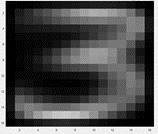
\includegraphics[width=0.55\linewidth]{mean_three.png}
		\caption{Mean image of digit 3}
		\label{fig:mean_three}
	\end{subfigure}
	\begin{subfigure}[b]{0.49\textwidth}
		\centering
		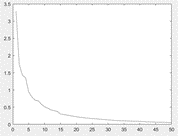
\includegraphics[width=0.6\linewidth]{50_largest_eigenvalues.png}
		\caption{Eigenvalues}
		\label{fig:50_largest_eigenvalues}
	\end{subfigure}
	\begin{subfigure}[b]{1.0\textwidth}
		\centering
		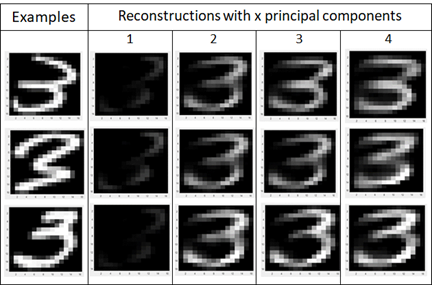
\includegraphics[width=0.4\linewidth]{reconstruction_x_principal_eigenvalues.png}
		\caption{Increasing amount of eigenvectors}
		\label{fig:increasing_eigenvectors}
	\end{subfigure}		
	\caption{Results of applying PCA on the US Postal Service database.}
	\label{fig:Results1}
\end{figure}

In Figure \ref{fig:Results2} the effect of the number of eigenvectors on the RMSE  used in the PCA, is investigated and the distribution of the sizes of the eigenvalues is shown. From Figure \ref{fig:Reconstruction_error1} it is concluded that when more eigenvectors are included, the representation error decreases because the dimensionality is less reduced. When the derivative of the function is assessed, it is found that the function decreases much faster at the beginning than at the end. This means that already by the use of a small amount of eigenvectors to span the subspace with a lower dimensionality, the reconstruction error can be significantly decreased and an already good reconstruction of the original data is possible. Figure \ref{fig:Reconstruction_error2} shows the cumulative sum of eigenvalues used in the PCA with on the x-axis the number of excluded eigenvalues starting from the largest. It is seen that a small amount of eigenvalues have large eigenvalues after which the size decreases rapidly. The plot is similar to Figure \ref{fig:Reconstruction_error1} and it can be concluded that the contribution of an eigenvector in reducing the RMSE corresponds to the size of the eigenvalue. This confirms what was concluded in Figure \ref{fig:Reconstruction_error1}, that already good representations of the digit 3 are possible with a small amount of eigenvectors. When Eq. \ref{eq:form1} is used without a dimensionality reduction, a very small reconstruction error equal to the default floating point precision in Matlab is found. 

\begin{figure}[h]
	\centering
	\begin{subfigure}[c]{0.49\textwidth}
		\centering
		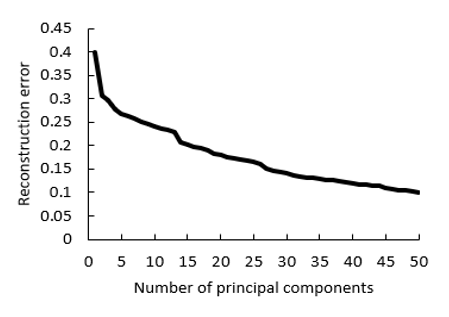
\includegraphics[width=0.85\linewidth]{Reconstruction_error1.png}
		\caption{}
		\label{fig:Reconstruction_error1}
	\end{subfigure}
	\begin{subfigure}[c]{0.49\textwidth}
		\centering
		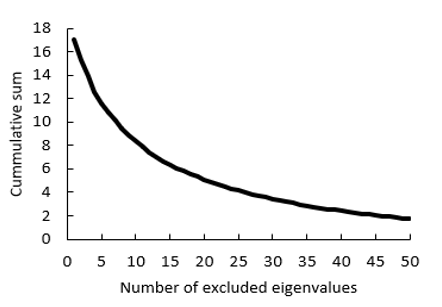
\includegraphics[width=0.8\linewidth]{Reconstruction_error2.png}
		\caption{}
		\label{fig:Reconstruction_error2}
	\end{subfigure}
	\caption{The influence of the amount of eigenvectors used.}
	\label{fig:Results2}
\end{figure}

\section{Stacked Autoencoders}
An autoencoder is an artificial network that learns efficient encodings of the original data. This is done to force the original data to be represented by only a limit amount of neurons causing a dimensionality reduction (encoding) after which the original data is reconstructed (decoding) and compared with the original inputs. When the outputs after decoding have a small reconstruction error, this means that the hidden layer that caused the dimensionality reduction, was able to identify the most important features that determine the data appearance. This is similarly as the goal of the principal component analysis. Stacked autoencoders refers to the sequential use of autoencoders where the hidden layer of a previous autoencoder serves as input of a next one. Applications of dimensionality reduction making use of autoencoders are:
\begin{itemize}
	\item Image compression
	\item Denoising
	\item Feature extraction
\end{itemize}

Image compression is used when storing images on a hard drive and an autoencoder can also be applied when preprocessing to remove noise. Here, the focus will be on feature extraction. By forcing a dimensionality reduction, the most important features of the original data are extracted and this is also desired by each layer in a conventional neural network. Therefore, a deep neural network can be efficiently trained one layer at a time where this layer is the hidden layer in an autoencoder. Features will be combined to obtain new features in deeper layers of the network. The training approach used is greedy layer-wise training which means sequentially learning the layers of the deep neural network using autoencoders which is unsupervised learning. A softmax layer is added for classification which is trained in a supervised manner. Finally, fine tuning is conducted which means that the total deep neural network is constructed and trained using labelled images. Next, the influence of different parameters is discussed. 

\subsection{MaxEpochs}
During training of the autoencoder, the softmax layer and fine-tuning the general rule of overfitting applies which states that: when a high number of epochs are trained, training error will decrease but the validation error will start to increase at a certain point in time. The point where the validation error starts to increase corresponds to the moment in time that the network stops learning general features from the inputs. Because it starts to remember specific aspects of the training data, this will not be general anymore and the error on unseen inputs i.e. the validation set, will increase. A suitable solution is to set a high value for MaxEpochs while monitoring the error on the validation set. This method is called early stopping and is by default applied in Matlab when applying supervised learning. 

\subsection{Number of hidden units}
The tradeoff that has to be made when choosing the amount of hidden neurons in the autoencoder is twofold. When the amount of neurons is selected too large, with as maximum equal to the amount of inputs, the dimensionality reduction is only small and the autoencoder is not pushed towards making satisfactory generalizations. This means that the learned hidden layer is very input specific with as extreme case that it just learns the identity function and no features are extracted. The reconstruction error will in this case be zero. On the other side, when a small amount of hidden units are selected, a very big dimensionality reduction is forced which causes the extracted features to be not representative for the inputs. This will give a large reconstruction error. The most suitable amount of hidden units is in the middle and problem specific. The amount of units chosen in the softmax layer corresponds to the amount of classes using a one hot encoding.

\subsection{Number of layers}
When more layers are used in the deep neural network the expressiveness of the model increases. Features will be combined to obtain new features in deeper layers of the network. Especially, when a model has a high expressiveness, extra care should be taken with overfitting. The increase of the amount of layers didn't give much improvement to the classification results. This indicates that the most relevant features used when classifying are already extracted in the first layer.\\ 

\subsection{Parameter tuning}
The default settings already very satisfactory results and have before fine-tuning a correct classification in $ 87.04\% $  and after fine-tuning in $ 99.74\% $ of the cases. Despite this, a small parameter search was conducted which varied the amount epochs, hidden units, and hidden layers. Every combination of values for the parameters is repeated 3 times in order to reduce the dependency of the results on the random weight initialisations. The best average run found has a correct classification of $ 98.88\% $ after fine-tuning.\\

Fine-tuning causes an additional increase of the correctness of classification around $ 10\% $ and is necessary if the the method using autoencoders wants to outperform the conventional way of training neural networks, which achieved a classification accuracy of $ 95.36\% $ and $ 97.24\%$ for respectively the use of one and two hidden layers. Fine-tuning is important because now the network is seen as a whole and the final classification error influences all the layers simultaneously by making use of back propagation. In comparison, first every hidden layer and softmax layer is trained individually. Only one hidden layer is needed together with 100 hidden units and 400 epochs to outperform the conventional neural networks. An average classification correctness was found of $ 98.88\% $ and fine-tuning only leads to an improvement of $ 0.28\% $.


%- autoencoder can also be used when training a deep neural network layer per layer. Each layer is supposed to learn features at a different level of abstraction. By using a sparse autoencoder, the layers are forced to reduce the dimensionality and learn important feature of the inputs. The hidden layer of the autoencoder, which corresponds to one of the hidden layers of the deep neural network is feeded as input of the next autoencoder. Using training with an autoencoder don't needs labels. A suitable solution is to make use of a validation set and early stopping. 

%- the number of layers --> the network becomes more expressive. Each layer can learn features at a different level of abstraction. This means that more care has to be taken with overfitting. A very expressive network doesn't make generalizations but remembers the training data. 
%
%- Fine-tuning is important because now the network is seen as a whole and the final classification error influences all the layers simultaneously by making use of back propagation. In comparison, first every hidden layer and softmax layer is trained individually. 




%\begin{table}
%	\centering
%	\begin{tabular}{@{}clr@{}} \toprule
%		\textbf{Attractor} & \textbf{Point} & \textbf{Stability}\\\midrule
%		Attractor $ 1 $ & $ [1;1] $ & Stable\\
%		Attractor $ 2 $ & $ [-1;-1] $ & Stable\\
%		Attractor $ 3 $ & $ [1;-1] $ & Stable\\
%		Attractor $ 4 $ & $ [-1;1] $ & Stable\\
%		Attractor $ 5 $ & $ [0;0] $ & Unstable\\
%		Attractor $ 6 $ & $ [0;1] $ & Unstable\\
%		Attractor $ 7 $ & $ [0;-1] $ & Unstable\\
%		Attractor $ 8 $ & $ [1;0] $ & Unstable\\
%		Attractor $ 9 $ & $ [-1;0] $ & Unstable\\\bottomrule
%	\end{tabular}
%	\caption{Overview of the different attractor points found in a 2D plane.}
%	\label{tab:att}
%\end{table}

\bibliographystyle{abbrv}
%\bibliography{ANN1}

\end{document}
